\documentclass[17pt]{extarticle}
\usepackage{tikz}
\usepackage{showexpl}
\usepackage{gensymb}
\usepackage{chemfig}
\usetikzlibrary{arrows.meta}
\usepackage[top=0.2in,left=0.9in,right=1cm]{geometry} %This geometry is page layout
\usepackage{titlesec}
\usepackage[utf8]{inputenc}
\title{Latex Diagram Referrence}
\author{For Mathematics}
\date{ }

\lstset
{   language=[LaTeX]TeX,
    breaklines=true,
    basicstyle=\fontsize{14}{14}\ttfamily,
    keywordstyle=\color{blue},
    identifierstyle=\color{magenta},
}

\begin{document}

\titleformat{\section}{\normalfont\normalsize\bfseries}{\thesection}{1em}{}
\titlespacing{\section}{0pt}{0pt}{-0.3 cm}  


%\maketitle
%\tableofcontents
%\pagebreak


%%%%%%%%%%%%%%%%%%%%%%%%%%%%%%%%%%%%%%%%%%%%%%%
%%%%%%%%%%%%%%%%%%%%%%%%%%%%%%%%%%%%%%%%%
%%%%%%%%%%%%%%%%%%%%%%%%%%%%%%%%%%%%%%%%%Start Examples
%%%%%%%%%%%%%%%%%%%%%%%%%%%%%%%%%%%%%%%%%
%%%%%%%%%%%%%%%%%%%%%%%%%%%%%%%%%%%%%%%%%

\section {Benzene Ring}

\begin{LTXexample}[pos=b,preset=\centering,width=1\linewidth]
  \vspace{5mm}
  \chemfig{*6(------)}
  \vspace{5mm}
\end{LTXexample}

\pagebreak

%%%%%%%%%%%%%%%%%%%%%%%%%%%%%%%%%%%%%%%%%%%%%%%%%%%%%%%%%%%%

\section {Bnezene Ring Double Bond}

\begin{LTXexample}[pos=b,preset=\centering,width=1\linewidth]
  \vspace{5mm}
  \chemfig{*6(=-=-=-)}
  \vspace{5mm}
\end{LTXexample}

\pagebreak

%%%%%%%%%%%%%%%%%%%%%%%%%%%%%%%%%%%%%%%%%%%%%%%
\section {Bond CH2}

\begin{LTXexample}[pos=b,preset=\centering,width=1\linewidth]
  \vspace{5mm}
  \chemfig{*6(---(-CH_2)-O--)}
  \vspace{5mm}
\end{LTXexample}

\pagebreak

%%%%%%%%%%%%%%%%%%%%%%%%%%%%%%%%%%%%%%%%%%%%%%%
\section {More Organic Compounds}

\begin{LTXexample}[pos=b,preset=\centering,width=1\linewidth]
  \vspace{5mm}
  \chemfig{A*6(-B=C(-CH_3)-D-E-F(=G)=)}
  \vspace{5mm}
\end{LTXexample}

\pagebreak

%%%%%%%%%%%%%%%%%%%%%%%%%%%%%%%%%%%%%%%%%%%%%%%%%%%%%%%%
\section {More Organic Compounds}

\begin{LTXexample}[pos=b,preset=\centering,width=1\linewidth]
  \vspace{5mm}
  \chemfig{*6(--*6(--*6(--*6(------)----)----)----)} 
  \vspace{5mm}
\end{LTXexample}
\pagebreak

%%%%%%%%%%%%%%%%%%%%%%%%%%%%%%%%%%%%%%%%%%%%%%%%%%%%%%%%

\section {More Organic Compounds}

\begin{LTXexample}[pos=b,preset=\centering,width=1\linewidth]
  \vspace{5mm}
  \definesubmol\Me[H_3C]{CH_3}
\chemfig{**6((-!\Me)=(-!\Me)-(-!\Me)=(-!\Me)-(-!\Me)=(-!\Me)-)}
  \vspace{5mm}
\end{LTXexample}
\pagebreak

%%%%%%%%%%%%%%%%%%%%%%%%%%%%%%%%%%%%%%%%%%%%%%%%%%%%%
\section {Cube - Unfolded}
\begin{LTXexample}[pos=b,preset=\centering,width=1\linewidth]
\vspace*{4mm} %to keep box edge little away
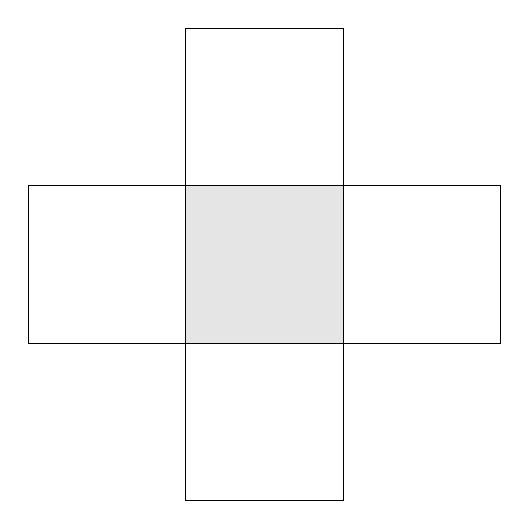
\begin{tikzpicture}
\draw (0,0) -- (0,2) -- (2,2) -- (2,4) -- (4,4) -- (4,2) -- (6,2) -- (6,0) -- (4,0) -- (4,-2) -- (2,-2) -- (2,0) -- (0,0) ; 
\filldraw[fill=gray!20] (2,0) rectangle (4,2);
\end{tikzpicture}
\vspace*{4mm} %to keep box edge little away
\end{LTXexample}
\pagebreak


\section {Cone}
\begin{LTXexample}[pos=b,preset=\centering,width=1\linewidth]
\vspace*{4mm} %to keep box edge little away
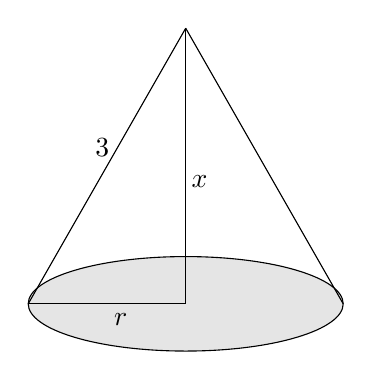
\begin{tikzpicture}
\filldraw[fill=gray!20](0,0) ellipse (2cm and 0.6cm);
\draw (0,0) -- node[below] {\ \ \ $x$}(0,3.5);
\draw (0,0)  -- node[below] {\ \ \ $r$} (-2,0);
\draw  (-2,0) --node[above] {3\ \ }(0,3.5);
\draw  (2,0) -- (0,3.5);
\end{tikzpicture}
\vspace*{4mm} %to keep box edge little away
\end{LTXexample}
\pagebreak
%%%%%%%%%%%%%%%%%%%%%%%%%%%%%%%%%%%%%%%
\section {Area Under The Curve}

\begin{LTXexample}[pos=b,preset=\centering,width=1\linewidth]
  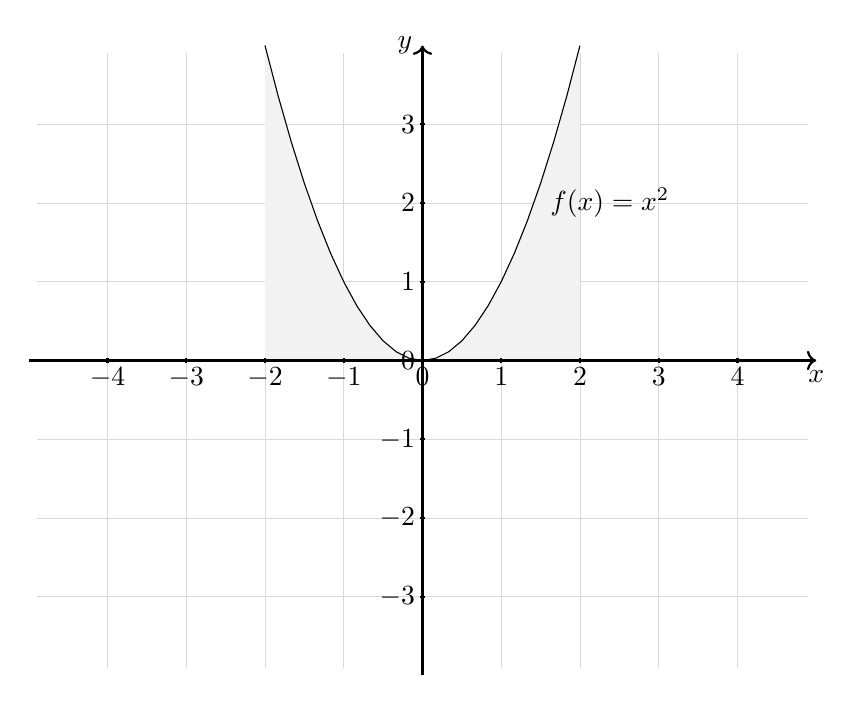
\begin{tikzpicture}
    \draw[very thin, gray!30, step=1 cm](-4.9,-3.9) grid (4.9,3.9);
    \fill [gray!10, domain=-2:2, variable=\x]
     (-2, 0) -- plot ({\x}, {\x*\x}) -- (2, 0) -- cycle;
    \draw [thick] [->] (-5,0)--(5,0) node[right, below] {$x$};
     \foreach \x in {-4,...,4}
       \draw[xshift=\x cm, thick] (0pt,-1pt)--(0pt,1pt) node[below] {$\x$};
      \draw [thick] [->] (0,-4)--(0,4) node[above, left] {$y$};
     \foreach \y in {-3,...,3}
       \draw[yshift=\y cm, thick] (-1pt,0pt)--(1pt,0pt) node[left] {$\y$};

    \draw [domain=-2:2, variable=\x]
      plot ({\x}, {\x*\x}) node[right] at (1.5,2) {$f(x)=x^2$};
  \end{tikzpicture}
\end{LTXexample}

\pagebreak

%%%%%%%%%%%%%%%%%%%%%%%%%%%%%%%%%%%%%%%%%%%%%%%%%%%%%%%%



\end{document}
